%%
%% Beginning of file 'sample.tex'
%%
%% Modified 2005 December 5
%%
%% This is a sample manuscript marked up using the
%% AASTeX v5.x LaTeX 2e macros.

%% The first piece of markup in an AASTeX v5.x document
%% is the \documentclass command. LaTeX will ignore
%% any data that comes before this command.

%% The command below calls the preprint style
%% which will produce a one-column, single-spaced document.
%% Examples of commands for other substyles follow. Use
%% whichever is most appropriate for your purposes.
%%
%%\documentclass[12pt,preprint]{aastex}

%% manuscript produces a one-column, double-spaced document:

%\documentclass[manuscript]{aastex}

%% preprint2 produces a double-column, single-spaced document:

\documentclass[preprint2]{emulateapj}

\usepackage{natbib}
\bibliographystyle{apj}
\usepackage{longtable}
\usepackage[]{graphicx}
\usepackage{amsmath}
\usepackage{natbib}
\usepackage{tabularx}
\usepackage{bm}
\usepackage{color}
\usepackage{hyperref}

%% Sometimes a paper's abstract is too long to fit on the
%% title page in preprint2 mode. When that is the case,
%% use the longabstract style option.

%% \documentclass[preprint2,longabstract]{aastex}

%% If you want to create your own macros, you can do so
%% using \newcommand. Your macros should appear before
%% the \begin{document} command.
%%
%% If you are submitting to a journal that translates manuscripts
%% into SGML, you need to follow certain guidelines when preparing
%% your macros. See the AASTeX v5.x Author Guide
%% for information.

\newcommand{\vdag}{(v)^\dagger}
\newcommand{\myemail}{gsavorgn@astro.swin.edu.au}

\newcommand{\fitfigurewidth}{0.8\textwidth}

%% You can insert a short comment on the title page using the command below.

%\slugcomment{Not to appear in Nonlearned J., 45.}

%% If you wish, you may supply running head information, although
%% this information may be modified by the editorial offices.
%% The left head contains a list of authors,
%% usually a maximum of three (otherwise use et al.).  The right
%% head is a modified title of up to roughly 44 characters.
%% Running heads will not print in the manuscript style.

\shorttitle{Mbh-n paper}
\shortauthors{Savorgnan et al.}

%% This is the end of the preamble.  Indicate the beginning of the
%% paper itself with \begin{document}.

\begin{document}

%% LaTeX will automatically break titles if they run longer than
%% one line. However, you may use \\ to force a line break if
%% you desire.

\title{Mbh-n paper}

%% Use \author, \affil, and the \and command to format
%% author and affiliation information.
%% Note that \email has replaced the old \authoremail command
%% from AASTeX v4.0. You can use \email to mark an email address
%% anywhere in the paper, not just in the front matter.
%% As in the title, use \\ to force line breaks.

\author{G. A. D. Savorgnan\altaffilmark{1} and A. W. Graham\altaffilmark{1}}
\affil{Centre for Astrophysics and Supercomputing, Swinburne University of Technology, Hawthorn, Victoria 3122, Australia.}

%\author{C. D. Biemesderfer\altaffilmark{4,5}}
%\affil{National Optical Astronomy Observatories, Tucson, AZ 85719}
\email{gsavorgn@astro.swin.edu.au}

%\and

%\author{A. W. Graham\altaffilmark{1}}
%\affil{Centre for Astrophysics and Supercomputing, Swinburne University of Technology, Hawthorn, Victoria 3122, Australia.}

%% Notice that each of these authors has alternate affiliations, which
%% are identified by the \altaffilmark after each name.  Specify alternate
%% affiliation information with \altaffiltext, with one command per each
%% affiliation.

%\altaffiltext{1}{Visiting Astronomer, Cerro Tololo Inter-American Observatory.
%CTIO is operated by AURA, Inc.\ under contract to the National Science
%Foundation.}
%\altaffiltext{2}{Society of Fellows, Harvard University.}
%\altaffiltext{3}{present address: Center for Astrophysics,
%    60 Garden Street, Cambridge, MA 02138}
%\altaffiltext{4}{Visiting Programmer, Space Telescope Science Institute}
%\altaffiltext{5}{Patron, Alonso's Bar and Grill}

%% Mark off your abstract in the ``abstract'' environment. In the manuscript
%% style, abstract will output a Received/Accepted line after the
%% title and affiliation information. No date will appear since the author
%% does not have this information. The dates will be filled in by the
%% editorial office after submission.

\begin{abstract}
blah blah
\end{abstract}


\keywords{keywords}


\section{Introduction}
The empirical \cite{sersic1963,1968} model has been demonstrated to provide adequate description 
of the light distribution of the stellar spheroidal component of galaxies, 
yet its physical intepretation has remained unknown for decades. 


origin of L-n \\
M-L + L-n ... M-n \\
M-C and M-n \\
s+11 v+12 b+12 \\
my paper \\
paper I and II \\


\section{Data}

\begin{table*}                                        
\begin{center}                                        
\caption{{\bf Galaxy sample.}                        
\emph{Column (1):} Galaxy name.                       
\emph{Column (2):} Distance.                                   
\emph{Column (3):} Black hole mass.                                   
\emph{Column (4):} Reference of the black hole mass reported here (G+03 = \citealt{greenhill2003}, GS13 = \citealt{grahamscott2013}; R+13b = \citealt{rusli2013bhmassesDM}).                                   
\emph{Column (5):} Presence of a partially depleted core. 
The question mark is used when the classification has come from the velocity dispersion criteria mentioned in Section \ref{sec:corser}. 
The value of the core break radius is reported in parenthesis when available.  
\emph{Column (6):} Reference of the identification of a partially depleted core (G+94 = \citealt{grillmair1994}; F+97 = \citealt{forbes1997}; Q+00 = \citealt{quillen2000}, 
T+04 = \citealt{trujillo2004coresersicmodel}; F+06 = \citealt{ferrarese2006acsvcs}; J+11 = \citealt{jardel2011}; R+11 = \citealt{richings2011}; 
DG13 = \citealt{dullograham2013cores}; R+13a = \citealt{rusli2013}).  
\emph{Column (7):} Kinematical classification (fast/slow rotator).
\emph{Column (8):} Availability of velocity map (A = ATLAS$^{\rm 3D}$, S = SLUGGS). 
\emph{Column (9):} Completion of 1D fit. 
\emph{Column (10):} Completion of 2D fit. }                                 
\begin{tabular}{llllllllll}                           
\hline                                                
\multicolumn{1}{l}{{\bf Galaxy}} &                   
\multicolumn{1}{l}{{\bf Distance}} &                 
\multicolumn{1}{l}{{\bf $\bm{M_{\rm BH}}$}} &  
\multicolumn{1}{l}{{\bf Ref.}} &                     
\multicolumn{1}{l}{{\bf Core}} &                     
\multicolumn{1}{l}{{\bf Ref.}} &                     
\multicolumn{1}{l}{{\bf Rot.}} &                     
\multicolumn{1}{l}{{\bf Vel. map}} &                 
\multicolumn{1}{l}{{\bf 1D fit}} &                   
\multicolumn{1}{l}{{\bf 2D fit}} \\                
\multicolumn{1}{l}{} &                                
\multicolumn{1}{l}{[Mpc]} &                           
\multicolumn{1}{l}{$[10^8~\rm M_{\odot}]$} &         
\multicolumn{1}{l}{} &                                
\multicolumn{1}{l}{$([\rm arcsec])$} &                                
\multicolumn{1}{l}{} &                                
\multicolumn{1}{l}{} &                                
\multicolumn{1}{l}{} &                                
\multicolumn{1}{l}{} &                                
\multicolumn{1}{l}{} \\                             
\multicolumn{1}{l}{(1)} &                             
\multicolumn{1}{l}{(2)} &                             
\multicolumn{1}{l}{(3)} &                             
\multicolumn{1}{l}{(4)} &                             
\multicolumn{1}{l}{(5)} &                             
\multicolumn{1}{l}{(6)} &                             
\multicolumn{1}{l}{(7)} &                             
\multicolumn{1}{l}{(8)} &                             
\multicolumn{1}{l}{(9)} &                             
\multicolumn{1}{l}{(10)} \\                         
\hline                                                
Circinus   &  $4.0$  &  $0.017_{-0.003}^{+0.004}$   &  G+03  &  no?  &     &      &     &  no  &  no  \\ 
IC 1459  &  $28.4$  &  $24_{-10}^{+10}$   &  GS13  &  yes  $(0.7)$  &  R+13a  &      &     &  yes  &  yes  \\ 
IC 2560  &  $40.7$  &  $0.044_{-0.022}^{+0.044}$   &  GS13  &  no?  &     &      &     &  yes  &  no  \\ 
IC 4296  &  $40.7$  &  $11_{-2}^{+2}$   &  GS13  &  yes?  &     &      &     &  yes  &  yes  \\ 
M104  &  $9.5$  &  $6.4_{-0.4}^{+0.4}$   &  GS13  &  yes   &  J+11  &      &     &  yes  &  no  \\ 
M105  &  $10.3$  &  $4_{-1}^{+1}$   &  GS13  &  yes  $(1.1)$  &  DG13, R+13a  &  FAST   &  A  &  yes  &  yes  \\ 
M106  &  $7.2$  &  $0.39_{-0.01}^{+0.01}$   &  GS13  &  no   &     &      &     &  yes  &  no  \\ 
M31  &  $0.7$  &  $1.4_{-0.3}^{+0.9}$   &  GS13  &  no   &     &      &     &  yes  &  no  \\ 
M32  &  $0.8$  &  $0.024_{-0.005}^{+0.005}$   &  GS13  &  no   &     &      &     &  no  &  no  \\ 
M49  &  $17.1$  &  $25_{-1}^{+3}$   &  R+13b  &  yes  $(1.5)$  &  DG13, R+13a  &   SLOW  &  A  &  yes  &  yes  \\ 
M59  &  $17.8$  &  $3.9_{-0.4}^{+0.4}$   &  GS13  &  no   &     &  FAST   &  A  &  yes  &  no  \\ 
M60  &  $16.4$  &  $47_{-10}^{+10}$   &  GS13  &  yes  $(2.7)$  &  DG13, R+13a  &  FAST   &  A, S  &  no  &  no  \\ 
M64  &  $7.3$  &  $0.016_{-0.004}^{+0.004}$   &  GS13  &  no?  &     &      &     &  yes  &  no  \\ 
M77  &  $15.2$  &  $0.084_{-0.003}^{+0.003}$   &  GS13  &  no   &     &      &     &  no  &  no  \\ 
M81  &  $3.8$  &  $0.74_{-0.11}^{+0.21}$   &  GS13  &  no   &     &      &     &  yes  &  no  \\ 
M84  &  $17.9$  &  $9.0_{-0.8}^{+0.9}$   &  GS13  &  yes  $(1.9)$  &  F+06  &   SLOW  &  A, S  &  yes  &  yes  \\ 
M87  &  $15.6$  &  $58.0_{-3.5}^{+3.5}$   &  GS13  &  yes  $(7.2)$  &  F+06  &   SLOW  &  A, S  &  yes  &  yes  \\ 
M89  &  $14.9$  &  $4.7_{-0.5}^{+0.5}$   &  GS13  &  yes  $(0.4)$  &  DG13, R+13a  &   SLOW  &  A  &  yes  &  no  \\ 
M94  &  $4.4$  &  $0.060_{-0.014}^{+0.014}$   &  GS13  &  no?  &     &      &     &  yes  &  no  \\ 
M96  &  $10.1$  &  $0.073_{-0.015}^{+0.015}$   &  GS13  &  no   &     &      &     &  yes  &  yes  \\ 
NGC 0253  &  $3.5$  &  $0.10_{-0.05}^{+0.10}$   &  GS13  &  no   &     &      &     &  no  &  no  \\ 
NGC 0524  &  $23.3$  &  $8.3_{-1.3}^{+2.7}$   &  GS13  &  yes  $(0.2)$  &  R+11  &  FAST   &  A  &  yes  &  no  \\ 
NGC 0821  &  $23.4$  &  $0.39_{-0.09}^{+0.26}$   &  GS13  &  no   &     &  FAST   &  A, S  &  yes  &  yes  \\ 
NGC 1023  &  $11.1$  &  $0.42_{-0.04}^{+0.04}$   &  GS13  &  no   &     &  FAST   &  A, S  &  yes  &  yes  \\ 
NGC 1300  &  $20.7$  &  $0.73_{-0.35}^{+0.69}$   &  GS13  &  no   &     &      &     &  yes  &  no  \\ 
NGC 1316  &  $18.6$  &  $1.50_{-0.80}^{+0.75}$   &  GS13  &  no   &     &  FAST   &     &  yes  &  no  \\ 
NGC 1332  &  $22.3$  &  $14_{-2}^{+2}$   &  GS13  &  no   &     &      &     &  yes  &  no  \\ 
NGC 1374  &  $19.2$  &  $5.8_{-0.5}^{+0.5}$   &  R+13b  &  no?  &     &  FAST   &  A  &  yes  &  yes  \\ 
NGC 1399  &  $19.4$  &  $4.7_{-0.6}^{+0.6}$   &  GS13  &  yes  $(2.4)$  &  DG13, R+13a  &   SLOW  &  A  &  yes  &  no  \\ 
NGC 2273  &  $28.5$  &  $0.083_{-0.004}^{+0.004}$   &  GS13  &  no   &     &      &     &  yes  &  no  \\ 
NGC 2549  &  $12.3$  &  $0.14_{-0.13}^{+0.02}$   &  GS13  &  no   &     &  FAST   &  A  &  yes  &  yes  \\ 
NGC 2778  &  $22.3$  &  $0.15_{-0.10}^{+0.09}$   &  GS13  &  no   &     &  FAST   &  A  &  yes  &  no  \\ 
NGC 2787  &  $7.3$  &  $0.40_{-0.05}^{+0.04}$   &  GS13  &  no   &     &      &     &  yes  &  no  \\ 
NGC 2974  &  $20.9$  &  $1.7_{-0.2}^{+0.2}$   &  GS13  &  no   &     &  FAST   &  A, S  &  yes  &  yes  \\ 
NGC 3079  &  $20.7$  &  $0.024_{-0.012}^{+0.024}$   &  GS13  &  no?  &     &      &     &  yes  &  no  \\ 
NGC 3091  &  $51.2$  &  $36_{-2}^{+1}$   &  R+13b  &  yes  $(0.6)$  &  R+13a  &      &     &  yes  &  yes  \\ 
NGC 3115  &  $9.4$  &  $8.8_{-2.7}^{+10.0}$   &  GS13  &  no   &     &      &     &  yes  &  no  \\ 
NGC 3227  &  $20.3$  &  $0.14_{-0.06}^{+0.10}$   &  GS13  &  no   &     &      &     &  yes  &  no  \\ 
NGC 3245  &  $20.3$  &  $2.0_{-0.5}^{+0.5}$   &  GS13  &  no   &     &  FAST   &  A  &  yes  &  yes  \\ 
NGC 3377  &  $10.9$  &  $0.77_{-0.06}^{+0.04}$   &  GS13  &  no   &     &  FAST   &  A, S  &  yes  &  yes  \\ 
NGC 3384  &  $11.3$  &  $0.17_{-0.02}^{+0.01}$   &  GS13  &  no   &     &  FAST   &  A  &  yes  &  no  \\ 
NGC 3393  &  $55.2$  &  $0.34_{-0.02}^{+0.02}$   &  GS13  &  no   &     &      &     &  yes  &  yes  \\ 
NGC 3414  &  $24.5$  &  $2.4_{-0.3}^{+0.3}$   &  GS13  &  no   &     &   SLOW  &  A  &  yes  &  no  \\ 
NGC 3489  &  $11.7$  &  $0.058_{-0.008}^{+0.008}$   &  GS13  &  no   &     &  FAST   &  A  &  yes  &  yes  \\ 
NGC 3585  &  $19.5$  &  $3.1_{-0.6}^{+1.4}$   &  GS13  &  no   &     &      &     &  yes  &  no  \\ 
NGC 3607  &  $22.2$  &  $1.3_{-0.5}^{+0.5}$   &  GS13  &  no   &     &  FAST   &  A  &  yes  &  yes  \\ 
NGC 3608  &  $22.3$  &  $2.0_{-0.6}^{+1.1}$   &  GS13  &  yes  $(0.2)$  &  DG13, R+13a  &   SLOW  &  A, S  &  yes  &  yes  \\ 
NGC 3842  &  $98.4$  &  $97_{-26}^{+30}$   &  GS13  &  yes  $(0.7)$  &  DG13, R+13a  &      &     &  yes  &  no  \\ 
NGC 3998  &  $13.7$  &  $8.1_{-1.9}^{+2.0}$   &  GS13  &  no   &     &  FAST   &  A  &  yes  &  no  \\ 
NGC 4026  &  $13.2$  &  $1.8_{-0.3}^{+0.6}$   &  GS13  &  no   &     &  FAST   &  A  &  yes  &  no  \\ 
NGC 4151  &  $20.0$  &  $0.65_{-0.07}^{+0.07}$   &  GS13  &  no   &     &      &     &  yes  &  no  \\ 
\hline         
\end{tabular}   
\label{tab:sample} 
\end{center}    
\end{table*}    

\begin{table*}                                        
\begin{center}                                        
\begin{tabular}{llllllllll}                           
\hline                                                
\multicolumn{1}{l}{{\bf Galaxy}} &                   
\multicolumn{1}{l}{{\bf Distance}} &                 
\multicolumn{1}{l}{{\bf $\mathbf{M_{\rm BH}}$}} &  
\multicolumn{1}{l}{{\bf Ref.}} &                     
\multicolumn{1}{l}{{\bf Core}} &                     
\multicolumn{1}{l}{{\bf Ref.}} &                     
\multicolumn{1}{l}{{\bf Rot.}} &                     
\multicolumn{1}{l}{{\bf Vel. map}} &                 
\multicolumn{1}{l}{{\bf 1D fit}} &                   
\multicolumn{1}{l}{{\bf 2D fit}} \\                
\multicolumn{1}{l}{} &                                
\multicolumn{1}{l}{[Mpc]} &                           
\multicolumn{1}{l}{$[10^8~\rm M_{\odot}]$} &         
\multicolumn{1}{l}{} &                                
\multicolumn{1}{l}{$([\rm arcsec])$} &                                
\multicolumn{1}{l}{} &                                
\multicolumn{1}{l}{} &                                
\multicolumn{1}{l}{} &                                
\multicolumn{1}{l}{} &                                
\multicolumn{1}{l}{} \\                             
\multicolumn{1}{l}{(1)} &                             
\multicolumn{1}{l}{(2)} &                             
\multicolumn{1}{l}{(3)} &                             
\multicolumn{1}{l}{(4)} &                             
\multicolumn{1}{l}{(5)} &                             
\multicolumn{1}{l}{(6)} &                             
\multicolumn{1}{l}{(7)} &                             
\multicolumn{1}{l}{(8)} &                             
\multicolumn{1}{l}{(9)} &                             
\multicolumn{1}{l}{(10)} \\                         
\hline                                                
NGC 4261  &  $30.8$  &  $5_{-1}^{+1}$   &  GS13  &  yes  $(1.6)$  &  R+11  &   SLOW  &  A  &  yes  &  yes  \\ 
NGC 4291  &  $25.5$  &  $3.3_{-2.5}^{+0.9}$   &  GS13  &  yes  $(0.3)$  &  DG13, R+13a  &      &     &  yes  &  yes  \\ 
NGC 4342  &  $23.0$  &  $4.5_{-1.5}^{+2.3}$   &  GS13  &  no   &     &  FAST   &  A  &  no  &  no  \\ 
NGC 4388  &  $17.0$  &  $0.075_{-0.002}^{+0.002}$   &  GS13  &  no?  &     &      &     &  yes  &  no  \\ 
NGC 4459  &  $15.7$  &  $0.68_{-0.13}^{+0.13}$   &  GS13  &  no   &     &  FAST   &  A  &  yes  &  no  \\ 
NGC 4473  &  $15.3$  &  $1.2_{-0.9}^{+0.4}$   &  GS13  &  no   &     &  FAST   &  A, S  &  yes  &  yes  \\ 
NGC 4486A  &  $17.0$  &  $0.13_{-0.08}^{+0.08}$   &  GS13  &  no   &     &  FAST   &  A  &  no  &  no  \\ 
NGC 4564  &  $14.6$  &  $0.60_{-0.09}^{+0.03}$   &  GS13  &  no   &     &  FAST   &  A  &  yes  &  no  \\ 
NGC 4596  &  $17.0$  &  $0.79_{-0.33}^{+0.38}$   &  GS13  &  no   &     &  FAST   &  A  &  yes  &  no  \\ 
NGC 4697  &  $11.4$  &  $1.8_{-0.1}^{+0.2}$   &  GS13  &  no   &     &  FAST   &  A, S  &  yes  &  yes  \\ 
NGC 4889  &  $103.2$  &  $210_{-160}^{+160}$   &  GS13  &  yes  $(1.7)$  &  F+97  &      &     &  yes  &  yes  \\ 
NGC 4945  &  $3.8$  &  $0.014_{-0.007}^{+0.014}$   &  GS13  &  no?  &     &      &     &  yes  &  yes  \\ 
NGC 5077  &  $41.2$  &  $7.4_{-3.0}^{+4.7}$   &  GS13  &  yes  $(0.3)$  &  T+04  &      &     &  yes  &  yes  \\ 
NGC 5128  &  $3.8$  &  $0.45_{-0.10}^{+0.17}$   &  GS13  &  no?  &     &      &     &  yes  &  no  \\ 
NGC 5576  &  $24.8$  &  $1.6_{-0.4}^{+0.3}$   &  GS13  &  no   &     &   SLOW  &  A  &  yes  &  yes  \\ 
NGC 5813  &  $31.3$  &  $6.8_{-0.7}^{+0.7}$   &  GS13  &  yes  $(0.4)$  &  DG13, R+13a  &   SLOW  &  A  &  no  &  no  \\ 
NGC 5845  &  $25.2$  &  $2.6_{-1.5}^{+0.4}$   &  GS13  &  no   &     &  FAST   &  A  &  yes  &  yes  \\ 
NGC 5846  &  $24.2$  &  $11_{-1}^{+1}$   &  GS13  &  yes   &  F+97  &   SLOW  &  A, S  &  yes  &  yes  \\ 
NGC 6251  &  $104.6$  &  $5_{-2}^{+2}$   &  GS13  &  yes?  &     &      &     &  yes  &  yes  \\ 
NGC 7052  &  $66.4$  &  $3.7_{-1.5}^{+2.6}$   &  GS13  &  yes  $(0.8)$  &  Q+00  &      &     &  yes  &  yes  \\ 
NGC 7582  &  $22.0$  &  $0.55_{-0.19}^{+0.26}$   &  GS13  &  no   &     &      &     &  no  &  no  \\ 
NGC 7619  &  $51.5$  &  $25_{-3}^{+8}$   &  R+13b  &  yes  $(0.5)$  &  DG13, R+13a  &      &     &  yes  &  no  \\ 
NGC 7768  &  $112.8$  &  $13_{-4}^{+5}$   &  GS13  &  yes   &  G+94  &      &     &  yes  &  no  \\ 
UGC 03789  &  $48.4$  &  $0.108_{-0.005}^{+0.005}$   &  GS13  &  no?  &     &      &     &  yes  &  no  \\ 
\hline         
\end{tabular}   
\end{center}    
\end{table*}    


\section{Results}


\begin{figure}[h]
\begin{center}
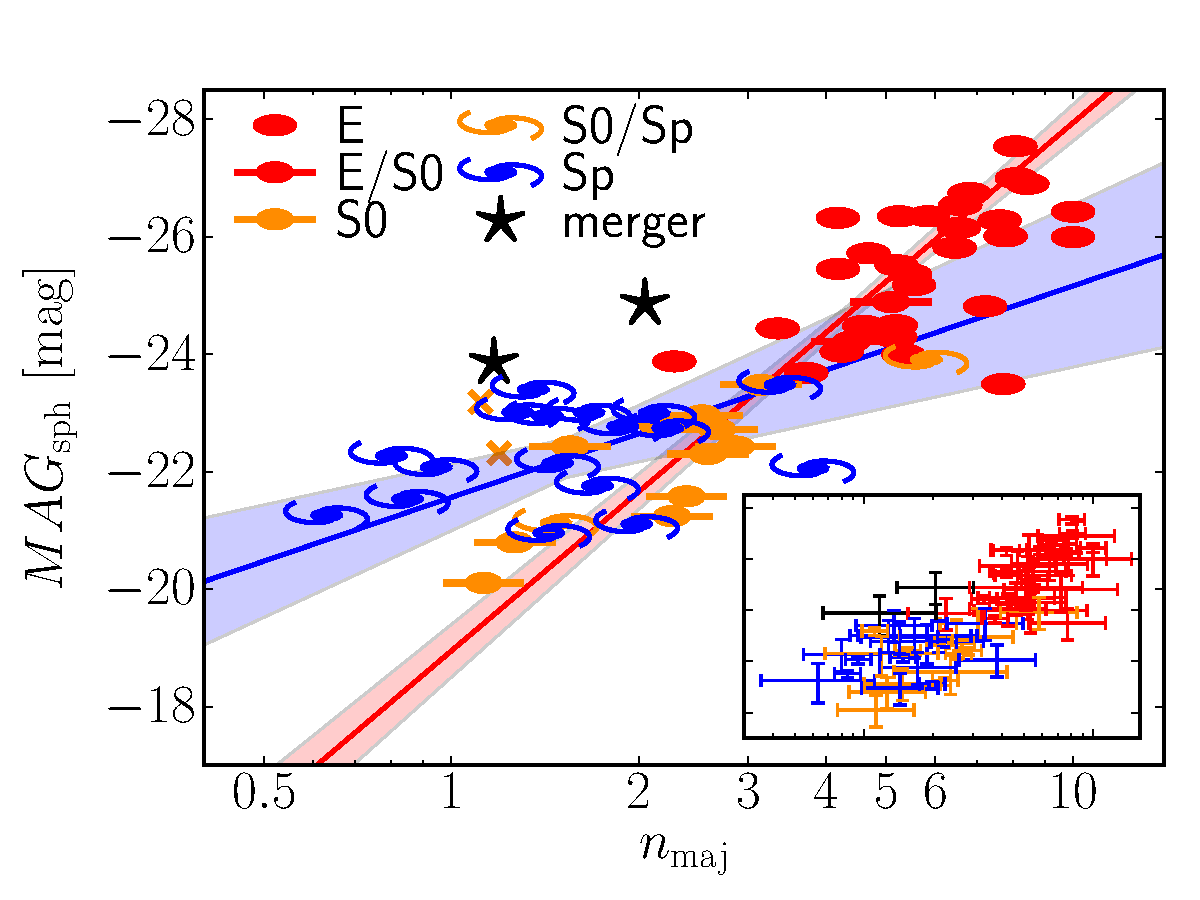
\includegraphics[width=\columnwidth]{images/mag_vs_n_maj.pdf}
\caption{}
\label{fig:magn}
\end{center}
\end{figure}

\begin{figure}[h]
\begin{center}
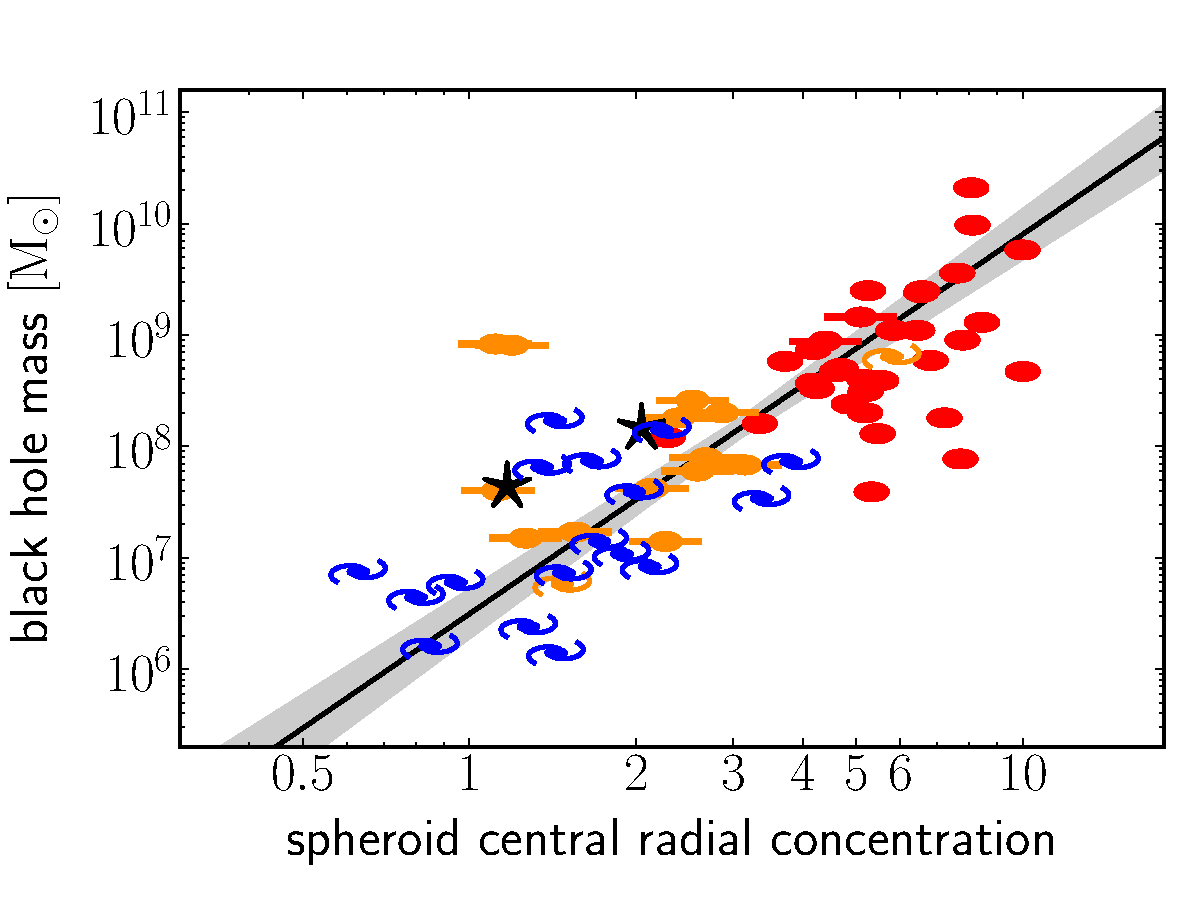
\includegraphics[width=\columnwidth]{images/mbh_vs_n_maj.pdf}
\caption{}
\label{fig:mbhn}
\end{center}
\end{figure}


\begin{table*}
\centering
\caption{Linear regression analysis of the $L_{\rm sph} - n_{\rm sph}$ diagram.}
\begin{tabular}{llccccc}
\tableline
\tableline
{\bf Subsample (size)} & {\bf Regression} & $\boldsymbol \alpha$ & $\boldsymbol \beta$ & $\boldsymbol \langle \log n_{\rm sph} \rangle$ & $\boldsymbol \epsilon$ & $\boldsymbol \Delta$ \\ 
\tableline 
\\
 & \multicolumn{6}{l}{$MAG_{\rm sph}/{\rm [mag]} = \alpha + \beta \bigl(\log n_{\rm sph} - \langle \log n_{\rm sph,maj} \rangle \bigr)$} \\ [0.5em]
All (62)               & BCES $(Y|X)$               & $-23.88 \pm 0.15$ & $-7.17 \pm 0.80$ & $0.51$ & $-$ & $1.18$ \\
                       & mFITEXY $(Y|X)$            & $-23.95 \pm 0.13$ & $-6.70 \pm 0.45$ & $0.51$ & $0.56^{+0.15}_{-0.10}$ & $0.98$ \\
                       & {\tt linmix\_err} $(Y|X)$  & $-23.92 \pm 0.15$ & $-6.40 \pm 0.57$ & $0.51$ & $0.74 \pm 0.13$ & $1.07$ \\ [0.5em]
                       & BCES $(X|Y)$               & $-23.88 \pm 0.14$ & $-6.70 \pm 0.51$ & $0.51$ & $-$ & $1.11$ \\
                       & mFITEXY $(X|Y)$            & $-23.94 \pm 0.14$ & $-7.50 \pm 0.52$ & $0.51$ & $0.59^{+0.17}_{-0.11}$ & $1.23$ \\
                       & {\tt linmix\_err} $(X|Y)$  & $-23.94 \pm 0.16$ & $-7.51 \pm 0.62$ & $0.51$ & $0.81 \pm 0.16$ & $1.23$ \\ [0.5em]
                       & BCES Bisector              & $-23.88 \pm 0.14$ & $-6.93 \pm 0.60$ & $0.51$ & $-$ & $1.14$ \\
                       & mFITEXY Bisector           & $-23.94 \pm 0.13$ & $-7.08 \pm 0.34$ & $0.51$ & $-$ & $1.16$ \\
                       & {\tt linmix\_err} Bisector & $-23.93 \pm 0.16$ & $-6.91 \pm 0.42$ & $0.51$ & $-$ & $1.14$ \\ [0.5em]

Elliptical (30)	       & BCES $(Y|X)$		    & $-25.46 \pm 1.12$ & $38.47 \pm 114.45$ & $0.76$ & $-$ & $6.37$ \\
		       & mFITEXY $(Y|X)$	    & $-25.74 \pm 0.18$ & $-9.74 \pm 1.59$ & $0.76$ & $0.24^{+0.32}_{-0.24}$ & $0.94$ \\
		       & {\tt linmix\_err} $(Y|X)$  & $-25.65 \pm 0.21$ & $-7.87 \pm 2.15$ & $0.76$ & $0.61 \pm 0.22$ & $1.06$ \\ [0.5em]
		       & BCES $(X|Y)$		    & $-25.46 \pm 0.23$ & $-10.73 \pm 3.21$ & $0.76$ & $-$ & $1.29$ \\
		       & mFITEXY $(X|Y)$	    & $-25.74 \pm 0.20$ & $-10.42 \pm 1.79$ & $0.76$ & $0.22^{+0.38}_{-0.22}$ & $1.29$ \\
		       & {\tt linmix\_err} $(X|Y)$  & $-25.72 \pm 0.28$ & $-10.92 \pm 2.70$ & $0.76$ & $0.73 \pm 0.34$ & $1.33$ \\ [0.5em]
		       & BCES Bisector  	    & $-25.46 \pm 0.20$ & $0.03 \pm 0.05$ & $0.76$ & $-$ & $1.14$ \\
		       & mFITEXY Bisector	    & $-25.74 \pm 0.19$ & $-10.07 \pm 1.19$ & $0.76$ & $-$ & $1.26$ \\
		       & {\tt linmix\_err} Bisector & $-25.68 \pm 0.25$ & $-9.15 \pm 1.74$ & $0.76$ & $-$ & $1.16$ \\ [0.5em]

Lenticular (11)	       & BCES $(Y|X)$		    & $-22.08 \pm 1.66$ & $33.52 \pm 98.87$ & $0.33$ & $-$ & $6.09$ \\
		       & mFITEXY $(Y|X)$	    & $-22.11 \pm 0.24$ & $-6.31 \pm 2.45$ & $0.33$ & $0.42^{+0.28}_{-0.17}$ & $0.71$ \\
		       & {\tt linmix\_err} $(Y|X)$  & $$ & $$ & $0.33$ & $$ & $$ \\ [0.5em]
		       & BCES $(X|Y)$		    & $-22.08 \pm 0.19$ & $-6.83 \pm 1.16$ & $0.33$ & $-$ & $0.71$ \\
		       & mFITEXY $(X|Y)$	    & $-21.94 \pm 0.44$ & $-13.16 \pm 7.91$ & $0.33$ & $0.61^{+0.60}_{-0.56}$ & $1.39$ \\
		       & {\tt linmix\_err} $(X|Y)$  & $$ & $$ & $0.33$ & $$ & $$ \\ [0.5em]
		       & BCES Bisector  	    & $-22.08 \pm 0.30$ & $0.06 \pm 0.05$ & $0.33$ & $-$ & $1.09$ \\
		       & mFITEXY Bisector	    & $-22.05 \pm 0.35$ & $-8.55 \pm 2.79$ & $0.33$ & $-$ & $0.84$ \\
		       & {\tt linmix\_err} Bisector & $$ & $$ & $0.33$ & $-$ & $$ \\ [0.5em]

Spiral (17)	       & BCES $(Y|X)$		    & $-22.33 \pm 0.26$ & $-5.31 \pm 5.83$ & $0.18$ & $-$ & $1.15$ \\
		       & mFITEXY $(Y|X)$	    & $-22.22 \pm 0.19$ & $-2.17 \pm 0.98$ & $0.18$ & $0.53^{+0.24}_{-0.13}$ & $0.72$ \\
		       & {\tt linmix\_err} $(Y|X)$  & $-22.26 \pm 0.24$ & $-1.53 \pm 1.88$ & $0.18$ & $0.71 \pm      0.22$ & $0.78$ \\ [0.5em]
		       & BCES $(X|Y)$		    & $-22.33 \pm 0.26$ & $-5.19 \pm 3.77$ & $0.18$ & $-$ & $1.13$ \\
		       & mFITEXY $(X|Y)$	    & $-22.28 \pm 0.44$ & $-9.08 \pm 5.31$ & $0.51$ & $1.12^{+0.54}_{-0.31}$ & $1.83$ \\
		       & {\tt linmix\_err} $(X|Y)$  & $-22.24 \pm 0.71$ & $-11.12 \pm 13.59$ & $0.18$ & $1.95 \pm 2.47$ & $2.24$ \\ [0.5em]
		       & BCES Bisector  	    & $-22.33 \pm 0.26$ & $-5.25 \pm 3.38$ & $0.18$ & $-$ & $1.14$ \\
		       & mFITEXY Bisector	    & $-22.23 \pm 0.33$ & $-3.60 \pm 1.29$ & $0.18$ & $-$ & $0.92$ \\
		       & {\tt linmix\_err} Bisector & $-22.25 \pm 0.53$ & $-2.88 \pm 2.66$ & $0.18$ & $-$ & $0.84$ \\ [0.5em]

\tableline 
\tableline
\end{tabular}
\end{table*}

\begin{table*}
\centering
\caption{Linear regression analysis of the $L_{\rm sph} - n_{\rm sph}$ diagram.}
\begin{tabular}{llccccc}
\tableline
\tableline
{\bf Subsample (size)} & {\bf Regression} & $\boldsymbol \alpha$ & $\boldsymbol \beta$ & $\boldsymbol \langle \log n_{\rm sph} \rangle$ & $\boldsymbol \epsilon$ & $\boldsymbol \Delta$ \\ 
\tableline 
\\
Early-type (43)	       & BCES $(Y|X)$		    & $-24.55 \pm 0.22$ & $-11.84 \pm 2.29$ & $0.64$ & $-$ & $1.50$ \\
		       & mFITEXY $(Y|X)$	    & $-24.74 \pm 0.14$ & $-8.86 \pm 0.66$ & $0.51$ & $0.27^{+0.20}_{-0.27}$ & $0.87$ \\
		       & {\tt linmix\_err} $(Y|X)$  & $-24.70 \pm 0.17$ & $-8.28 \pm 0.87$ & $0.64$ & $0.58 \pm 0.17$ & $0.98$ \\ [0.5em]
		       & BCES $(X|Y)$		    & $-24.55 \pm 0.14$ & $-8.25 \pm 0.63$ & $0.64$ & $-$ & $0.96$ \\
		       & mFITEXY $(X|Y)$	    & $-24.74 \pm 0.14$ & $-9.13 \pm 0.68$ & $0.64$ & $0.23^{+0.25}_{-0.23}$ & $1.08$ \\
		       & {\tt linmix\_err} $(X|Y)$  & $-24.73 \pm 0.18$ & $-9.08 \pm 0.87$ & $0.64$ & $0.60 \pm 0.21$ & $1.07$ \\ [0.5em]
		       & BCES Bisector  	    & $-24.55 \pm 0.17$ & $-9.73 \pm 1.05$ & $0.64$ & $-$ & $1.14$ \\
		       & mFITEXY Bisector	    & $-24.74 \pm 0.14$ & $-8.99 \pm 0.48$ & $0.64$ & $-$ & $1.06$ \\
		       & {\tt linmix\_err} Bisector & $-24.72 \pm 0.17$ & $-8.66 \pm 0.63$ & $0.64$ & $-$ & $1.02$ \\ [0.5em]

Bulge  (30)	       & BCES $(Y|X)$		    & $-22.25 \pm 0.20$ & $-5.88 \pm 3.06$ & $0.26$ & $-$ & $1.16$ \\
		       & mFITEXY $(Y|X)$	    & $-22.19 \pm 0.14$ & $-2.99 \pm 0.73$ & $0.26$ & $0.52^{+0.18}_{-0.10}$ & $0.75$ \\
		       & {\tt linmix\_err} $(Y|X)$  & $-22.20 \pm 0.17$ & $-2.48 \pm 1.21$ & $0.26$ & $0.67 \pm 0.15$ & $0.83$ \\ [0.5em]
		       & BCES $(X|Y)$		    & $-22.25 \pm 0.20$ & $-5.85 \pm 1.83$ & $0.26$ & $-$ & $1.15$ \\
		       & mFITEXY $(X|Y)$	    & $-22.17 \pm 0.25$ & $-7.65 \pm 2.43$ & $0.26$ & $0.87^{+0.30}_{-0.18}$ & $1.46$ \\
		       & {\tt linmix\_err} $(X|Y)$  & $-22.16 \pm 0.31$ & $-7.80 \pm 3.89$ & $0.26$ & $1.18 \pm 0.65$ & $1.48$ \\ [0.5em]
		       & BCES Bisector  	    & $-22.25 \pm 0.20$ & $-5.87 \pm 2.06$ & $0.26$ & $-$ & $1.16$ \\
		       & mFITEXY Bisector	    & $-22.18 \pm 0.20$ & $-4.34 \pm 0.84$ & $0.26$ & $-$ & $0.96$ \\
		       & {\tt linmix\_err} Bisector & $-22.19 \pm 0.25$ & $-3.83 \pm 1.39$ & $0.26$ & $-$ & $0.91$ \\ [1.0em]

% & \multicolumn{6}{l}{$MAG_{\rm sph}/{\rm [mag]} = \alpha + \beta \bigl(\log n_{\rm sph,eq} - \langle \log n_{\rm sph,eq} \rangle \bigr)$} \\ [0.5em]
%
% All (62)		 & BCES $(Y|X)$ 	      & $-23.88 \pm 0.15$ & $-7.04 \pm 0.89$ & $0.50$ & $-$ & $1.19$ \\
%			 & mFITEXY $(Y|X)$	      & $-23.95 \pm 0.12$ & $-6.43 \pm 0.41$ & $0.50$ & $0.55^{+0.16}_{-0.10}$ & $0.96$ \\
%			 & {\tt linmix\_err} $(Y|X)$  & $-23.91 \pm 0.14$ & $-6.04 \pm 0.54$ & $0.50$ & $0.75 \pm 0.13$ & $1.07$ \\ [0.5em]
%			 & BCES $(X|Y)$ 	      & $-23.88 \pm 0.14$ & $-6.73 \pm 0.48$ & $0.50$ & $-$ & $1.14$ \\
%			 & mFITEXY $(X|Y)$	      & $-23.93 \pm 0.13$ & $-7.13 \pm 0.48$ & $0.50$ & $0.58^{+0.17}_{-0.12}$ & $1.21$ \\
%			 & {\tt linmix\_err} $(X|Y)$  & $-23.93 \pm 0.15$ & $-7.14 \pm 0.57$ & $0.50$ & $0.76 \pm 0.16$ & $1.21$ \\ [0.5em]
%			 & BCES Bisector	      & $-23.88 \pm 0.15$ & $-6.88 \pm 0.62$ & $0.50$ & $-$ & $1.17$ \\
%			 & mFITEXY Bisector	      & $-23.94 \pm 0.13$ & $-6.76 \pm 0.31$ & $0.50$ & $-$ & $1.15$ \\
%			 & {\tt linmix\_err} Bisector & $-23.92 \pm 0.15$ & $-6.55 \pm 0.40$ & $0.50$ & $-$ & $1.12$ \\ [0.5em]
%
%
% Elliptical (30)	 & BCES $(Y|X)$ 	      & $-25.46 \pm 0.26$ & $4.92 \pm 4.72$ & $0.77$ & $-$ & $1.46$ \\
%			 & mFITEXY $(Y|X)$	      & $-25.66 \pm 0.24$ & $-12.65 \pm 2.78$ & $0.77$ & $0.42^{+0.38}_{-0.42}$ & $1.27$ \\
%			 & {\tt linmix\_err} $(Y|X)$  & $-25.55 \pm 0.26$ & $-8.54 \pm 4.68$ & $0.77$ & $0.80 \pm 0.24$ & $1.20$ \\ [0.5em]
%			 & BCES $(X|Y)$ 	      & $-25.46 \pm 0.40$ & $-20.83 \pm 11.31$ & $0.77$ & $-$ & $2.26$ \\
%			 & mFITEXY $(X|Y)$	      & $-25.63 \pm 0.31$ & $-16.13 \pm 4.37$ & $0.77$ & $0.48^{+0.48}_{-0.48}$ & $1.80$ \\
%			 & {\tt linmix\_err} $(X|Y)$  & $-25.63 \pm 0.43$ & $-16.66 \pm 6.50$ & $0.77$ & $1.22 \pm 0.65$ & $1.85$ \\ [0.5em]
%			 & BCES Bisector	      & $-25.46 \pm 0.20$ & $-0.08 \pm 0.10$ & $0.77$ & $-$ & $1.14$ \\
%			 & mFITEXY Bisector	      & $-25.65 \pm 0.28$ & $-14.18 \pm 2.43$ & $0.77$ & $-$ & $1.63$ \\
%			 & {\tt linmix\_err} Bisector & $-25.58 \pm 0.35$ & $-11.30 \pm 4.34$ & $0.77$ & $-$ & $1.38$ \\ [0.5em]
%
%\tableline 
%\tableline
%\end{tabular}
%\end{table*}
%
%\begin{table*}
%\centering
%\caption{Linear regression analysis of the $L_{\rm sph} - n_{\rm sph}$ diagram.}
%\begin{tabular}{llccccc}
%\tableline
%\tableline
%{\bf Subsample (size)} & {\bf Regression} & $\boldsymbol \alpha$ & $\boldsymbol \beta$ & $\boldsymbol \langle \log n_{\rm sph} \rangle$ & $\boldsymbol \epsilon$ & $\boldsymbol \Delta$ \\ 
%\tableline 
%\\
%
% Lenticular (11)	 & BCES $(Y|X)$ 	      & $-22.08 \pm 0.89$ & $16.29 \pm 24.44$ & $0.29$ & $-$ & $3.25$ \\
%			 & mFITEXY $(Y|X)$	      & $-22.16 \pm 0.20$ & $-5.84 \pm 1.83$ & $0.29$ & $0.31^{+0.28}_{-0.20}$ & $0.61$ \\
%			 & {\tt linmix\_err} $(Y|X)$  & $$ & $$ & $0.29$ & $$ & $$ \\ [0.5em]
%			 & BCES $(X|Y)$ 	      & $-22.08 \pm 0.20$ & $-7.40 \pm 1.27$ & $0.29$ & $-$ & $0.72$ \\
%			 & mFITEXY $(X|Y)$	      & $-22.11 \pm 0.28$ & $-8.30 \pm 3.33$ & $0.29$ & $0.40^{+0.33}_{-0.35}$ & $0.77$ \\
%			 & {\tt linmix\_err} $(X|Y)$  & $$ & $$ & $0.29$ & $$ & $$ \\ [0.5em]
%			 & BCES Bisector	      & $-22.08 \pm 0.30$ & $0.04 \pm 0.05$ & $0.29$ & $-$ & $1.08$ \\
%			 & mFITEXY Bisector	      & $-22.14 \pm 0.25$ & $-6.86 \pm 1.70$ & $0.29$ & $-$ & $0.70$ \\
%			 & {\tt linmix\_err} Bisector & $$ & $$ & $0.29$ & $$ & $$ \\ [0.5em]
%
%
% Spiral (17)		 & BCES $(Y|X)$ 	      & $-22.33 \pm 0.62$ & $-14.53 \pm 71.43$ & $0.17$ & $-$ & $2.71$ \\
%			 & mFITEXY $(Y|X)$	      & $-22.37 \pm 0.27$ & $-6.53 \pm 2.84$ & $0.17$ & $0.47^{+0.52}_{-0.39}$ & $0.95$ \\
%			 & {\tt linmix\_err} $(Y|X)$  & $-22.35 \pm 1.23$ & $-3.62 \pm 21.94$ & $0.17$ & $0.63 \pm 0.25$ & $0.93$ \\ [0.5em]
%			 & BCES $(X|Y)$ 	      & $-22.33 \pm 0.35$ & $-7.91 \pm 5.53$ & $0.17$ & $-$ & $1.54$ \\
%			 & mFITEXY $(X|Y)$	      & $-22.74 \pm 0.56$ & $-14.91 \pm 10.03$ & $0.17$ & $0.65^{+1.41}_{-0.65}$ & $2.82$ \\
%			 & {\tt linmix\_err} $(X|Y)$  & $-22.66 \pm 0.88$ & $-16.17 \pm 21.34$ & $0.17$ & $1.47 \pm 2.15$ & $3.04$ \\ [0.5em]
%			 & BCES Bisector	      & $-22.33 \pm 0.44$ & $-10.25 \pm 18.84$ & $0.17$ & $-$ & $1.94$ \\
%			 & mFITEXY Bisector	      & $-22.48 \pm 0.44$ & $-9.10 \pm 3.31$ & $0.17$ & $-$ & $1.75$ \\
%			 & {\tt linmix\_err} Bisector & $-22.41 \pm 1.07$ & $-5.98 \pm 28.65$ & $0.17$ & $-$ & $1.24$ \\ [0.5em]
%
%
% Early-type (43)	 & BCES $(Y|X)$ 	      & $-24.55 \pm 0.22$ & $-10.81 \pm 1.96$ & $0.64$ & $-$ & $1.46$ \\
%			 & mFITEXY $(Y|X)$	      & $-24.70 \pm 0.14$ & $-7.89 \pm 0.63$ & $0.64$ & $0.46^{+0.18}_{-0.14}$ & $0.93$ \\
%			 & {\tt linmix\_err} $(Y|X)$  & $-24.63 \pm 0.18$ & $-7.34 \pm 0.83$ & $0.64$ & $0.75 \pm 0.16$ & $1.02$ \\ [0.5em]
%			 & BCES $(X|Y)$ 	      & $-24.55 \pm 0.16$ & $-8.35 \pm 0.68$ & $0.64$ & $-$ & $1.10$ \\
%			 & mFITEXY $(X|Y)$	      & $-24.69 \pm 0.16$ & $-8.65 \pm 0.73$ & $0.64$ & $0.48^{+0.20}_{-0.15}$ & $1.14$ \\
%			 & {\tt linmix\_err} $(X|Y)$  & $-24.68 \pm 0.20$ & $-8.68 \pm 0.91$ & $0.64$ & $0.77 \pm 0.20$ & $1.14$ \\ [0.5em]
%			 & BCES Bisector	      & $-24.55 \pm 0.18$ & $-9.42 \pm 1.00$ & $0.64$ & $-$ & $1.23$ \\
%			 & mFITEXY Bisector	      & $-24.69 \pm 0.15$ & $-8.25 \pm 0.48$ & $0.64$ & $-$ & $1.10$ \\
%			 & {\tt linmix\_err} Bisector & $-24.65 \pm 0.19$ & $-7.96 \pm 0.62$ & $0.64$ & $-$ & $1.07$ \\ [0.5em]
%
%
% Bulge (30)		 & BCES $(Y|X)$ 	      & $-22.25 \pm 0.50$ & $-16.91 \pm 33.45$ & $0.23$ & $-$ & $2.85$ \\
%			 & mFITEXY $(Y|X)$	      & $-22.21 \pm 0.14$ & $-4.25 \pm 0.94$ & $0.23$ & $0.45^{+0.21}_{-0.13}$ & $0.75$ \\
%			 & {\tt linmix\_err} $(Y|X)$  & $-22.23 \pm 0.17$ & $-3.36 \pm 1.62$ & $0.23$ & $0.61 \pm 0.17$ & $0.87$ \\ [0.5em]
%			 & BCES $(X|Y)$ 	      & $-22.25 \pm 0.23$ & $-7.56 \pm 1.94$ & $0.23$ & $-$ & $1.30$ \\
%			 & mFITEXY $(X|Y)$	      & $-22.23 \pm 0.22$ & $-8.20 \pm 2.44$ & $0.23$ & $0.63^{+0.31}_{-0.19}$ & $1.39$ \\
%			 & {\tt linmix\_err} $(X|Y)$  & $-22.22 \pm 0.28$ & $-8.42 \pm 4.00$ & $0.23$ & $0.96 \pm 0.54$ & $1.43$ \\ [0.5em]
%			 & BCES Bisector	      & $-22.25 \pm 0.31$ & $-10.46 \pm 7.05$ & $0.23$ & $-$ & $1.75$ \\
%			 & mFITEXY Bisector	      & $-22.22 \pm 0.19$ & $-5.62 \pm 0.99$ & $0.23$ & $-$ & $1.05$ \\
%			 & {\tt linmix\_err} Bisector & $-22.23 \pm 0.23$ & $-4.84 \pm 1.75$ & $0.23$ & $-$ & $0.98$ \\ [0.5em]


%All (xx)		& BCES $(Y|X)$  	     & $$ & $$ & $$ & $$ & $$ \\
%			& mFITEXY $(Y|X)$	     & $$ & $$ & $$ & $$ & $$ \\
%			& {\tt linmix\_err} $(Y|X)$  & $$ & $$ & $$ & $$ & $$ \\ [0.5em]
%			& BCES $(X|Y)$  	     & $$ & $$ & $$ & $$ & $$ \\
%			& mFITEXY $(X|Y)$	     & $$ & $$ & $$ & $$ & $$ \\
%			& {\tt linmix\_err} $(X|Y)$  & $$ & $$ & $$ & $$ & $$ \\ [0.5em]
%			& BCES Bisector 	     & $$ & $$ & $$ & $$ & $$ \\
%			& mFITEXY Bisector	     & $$ & $$ & $$ & $$ & $$ \\
%			& {\tt linmix\_err} Bisector & $$ & $$ & $$ & $$ & $$ \\ [0.5em]
%

\tableline 
\tableline
\end{tabular}
\label{tab:lregLn} 
\tablecomments{For each subsample, we indicate $\langle \log n_{\rm sph} \rangle$, its average value of spheroid S\'ersic index. 
In the last two columns, we report $\epsilon$, the intrinsic scatter, and $\Delta$, the total rms scatter in the $L_{\rm sph}$ direction. 
all - mergers - outliers
Both the early- and late-type subsamples do not contain the two galaxies classified as S0/Sp and the two galaxies classified as mergers (45+17=66-2-2). }
\end{table*}


\begin{table*}
\centering
\caption{Linear regression analysis of the $M_{\rm BH} - n_{\rm sph}$ diagram.}
\begin{tabular}{llccccc}
\tableline
\tableline
{\bf Subsample (size)} & {\bf Regression} & $\boldsymbol \alpha$ & $\boldsymbol \beta$ & $\boldsymbol \langle \log n_{\rm sph} \rangle$ & $\boldsymbol \epsilon$ & $\boldsymbol \Delta$ \\ 
\tableline 
\\
 & \multicolumn{6}{l}{$\log \bigl( M_{\rm BH}/{\rm [M_\odot]} \bigr) = \alpha + \beta \bigl(\log n_{\rm sph} - \langle \log n_{\rm sph} \rangle \bigr)$} \\ [0.5em]
 All (62)		& BCES $(Y|X)$  	     & $8.14 \pm 0.08$ & $3.56 \pm 0.38$ & $0.51$ & $-$ & $0.60$ \\
 			& mFITEXY $(Y|X)$	     & $8.18 \pm 0.06$ & $3.27 \pm 0.21$ & $0.51$ & $0.22^{+0.10}_{-0.07}$ & $0.45$ \\
 			& {\tt linmix\_err} $(Y|X)$  & $8.17 \pm 0.06$ & $3.17 \pm 0.24$ & $0.51$ & $0.29 \pm 0.07$ & $0.56$ \\ [0.5em]
 			& BCES $(X|Y)$  	     & $8.14 \pm 0.08$ & $3.56 \pm 0.25$ & $0.51$ & $-$ & $0.60$ \\
 			& mFITEXY $(X|Y)$	     & $8.18 \pm 0.06$ & $3.51 \pm 0.23$ & $0.51$ & $0.23^{+0.10}_{-0.07}$ & $0.60$ \\
 			& {\tt linmix\_err} $(X|Y)$  & $8.17 \pm 0.07$ & $3.49 \pm 0.26$ & $0.51$ & $0.30 \pm 0.07$ & $0.60$ \\ [0.5em]
 			& BCES Bisector 	     & $8.14 \pm 0.08$ & $3.56 \pm 0.29$ & $0.51$ & $-$ & $0.60$ \\
 			& mFITEXY Bisector	     & $8.18 \pm 0.06$ & $3.39 \pm 0.15$ & $0.51$ & $-$ & $0.58$ \\
 			& {\tt linmix\_err} Bisector & $8.17 \pm 0.07$ & $3.33 \pm 0.18$ & $0.51$ & $-$ & $0.57$ \\ [0.5em]

 Elliptical (30)	& BCES $(Y|X)$  	     & $8.80 \pm 0.53$ & $-18.16 \pm 53.99$ & $0.76$ & $-$ & $3.02$ \\
 			& mFITEXY $(Y|X)$	     & $8.90 \pm 0.10$ & $4.47 \pm 0.88$ & $0.76$ & $0.29^{+0.14}_{-0.10}$ & $0.56$ \\
 			& {\tt linmix\_err} $(Y|X)$  & $8.84 \pm 0.12$ & $3.56 \pm 1.35$ & $0.76$ & $0.44 \pm 0.12$ & $0.59$ \\ [0.5em]
 			& BCES $(X|Y)$  	     & $8.80 \pm 0.18$ & $8.00 \pm 2.55$ & $0.76$ & $-$ & $1.01$ \\
 			& mFITEXY $(X|Y)$	     & $8.92 \pm 0.15$ & $6.85 \pm 1.75$ & $0.76$ & $0.36^{+0.20}_{-0.15}$ & $0.89$ \\
 			& {\tt linmix\_err} $(X|Y)$  & $8.89 \pm 0.20$ & $6.96 \pm 2.49$ & $0.76$ & $0.63 \pm 0.30$ & $0.89$ \\ [0.5em]
 			& BCES Bisector 	     & $8.80 \pm 0.11$ & $-0.03 \pm 0.10$ & $0.76$ & $-$ & $0.64$ \\
 			& mFITEXY Bisector	     & $8.91 \pm 0.13$ & $5.42 \pm 0.85$ & $0.76$ & $-$ & $0.73$ \\
 			& {\tt linmix\_err} Bisector & $8.85 \pm 0.16$ & $4.73 \pm 1.30$ & $0.76$ & $-$ & $0.67$ \\ [0.5em]

 Lenticular (11)	& BCES $(Y|X)$  	     & $7.75 \pm 0.58$ & $-11.51 \pm 31.78$ & $0.33$ & $-$ & $2.11$ \\
 			& mFITEXY $(Y|X)$	     & $7.65 \pm 0.12$ & $3.78 \pm 1.20$ & $0.33$ & $0.00^{+0.00}_{-0.00}$ & $0.26$ \\
 			& {\tt linmix\_err} $(Y|X)$  & $$ & $$ & $0.33$ & $$ & $$ \\ [0.5em]
 			& BCES $(X|Y)$  	     & $7.75 \pm 0.13$ & $3.54 \pm 0.99$ & $0.33$ & $-$ & $0.46$ \\
 			& mFITEXY $(X|Y)$	     & $7.65 \pm 0.12$ & $3.78 \pm 1.20$ & $0.33$ & $0.00^{+0.00}_{-0.00}$ & $0.49$ \\
 			& {\tt linmix\_err} $(X|Y)$  & $$ & $$ & $0.33$ & $$ & $$ \\ [0.5em]
 			& BCES Bisector 	     & $7.75 \pm 0.13$ & $-0.09 \pm 0.15$ & $0.33$ & $-$ & $0.48$ \\
 			& mFITEXY Bisector	     & $7.65 \pm 0.12$ & $3.78 \pm 0.85$ & $0.33$ & $-$ & $0.49$ \\
 			& {\tt linmix\_err} Bisector & $$ & $$ & $0.33$ & $-$ & $$ \\ [0.5em]

 Spiral (17)		& BCES $(Y|X)$  	     & $7.18 \pm 0.28$ & $6.78 \pm 6.62$ & $0.18$ & $-$ & $1.23$ \\
 			& mFITEXY $(Y|X)$	     & $7.24 \pm 0.13$ & $4.48 \pm 0.90$ & $0.18$ & $0.13^{+0.42}_{-0.13}$ & $0.52$ \\
 			& {\tt linmix\_err} $(Y|X)$  & $7.22 \pm 0.16$ & $3.57 \pm 1.36$ & $0.18$ & $0.39 \pm 0.19$ & $0.70$ \\ [0.5em]
 			& BCES $(X|Y)$  	     & $7.18 \pm 0.23$ & $5.48 \pm 1.93$ & $0.18$ & $-$ & $0.99$ \\
 			& mFITEXY $(X|Y)$	     & $7.24 \pm 0.14$ & $4.62 \pm 0.96$ & $0.18$ & $0.13^{+0.43}_{-0.13}$ & $0.85$ \\
 			& {\tt linmix\_err} $(X|Y)$  & $7.21 \pm 0.21$ & $4.86 \pm 1.64$ & $0.18$ & $0.45 \pm 0.31$ & $0.89$ \\ [0.5em]
 			& BCES Bisector 	     & $7.18 \pm 0.25$ & $6.06 \pm 3.66$ & $0.18$ & $-$ & $1.10$ \\
 			& mFITEXY Bisector	     & $7.24 \pm 0.14$ & $4.55 \pm 0.66$ & $0.18$ & $-$ & $0.84$ \\
 			& {\tt linmix\_err} Bisector & $7.22 \pm 0.19$ & $4.12 \pm 1.07$ & $0.18$ & $-$ & $0.77$ \\ [0.5em]

 Early-type (43)	& BCES $(Y|X)$  	     & $8.54 \pm 0.10$ & $4.07 \pm 0.87$ & $0.64$ & $-$ & $0.65$ \\
 			& mFITEXY $(Y|X)$	     & $8.58 \pm 0.07$ & $3.32 \pm 0.34$ & $0.64$ & $0.24^{+0.10}_{-0.07}$ & $0.45$ \\
 			& {\tt linmix\_err} $(Y|X)$  & $8.57 \pm 0.08$ & $3.12 \pm 0.43$ & $0.64$ & $0.32 \pm 0.08$ & $0.53$ \\ [0.5em]
 			& BCES $(X|Y)$  	     & $8.54 \pm 0.09$ & $3.95 \pm 0.55$ & $0.64$ & $-$ & $0.63$ \\
 			& mFITEXY $(X|Y)$	     & $8.59 \pm 0.08$ & $3.88 \pm 0.43$ & $0.64$ & $0.26^{+0.11}_{-0.08}$ & $0.62$ \\
 			& {\tt linmix\_err} $(X|Y)$  & $8.59 \pm 0.09$ & $3.82 \pm 0.50$ & $0.64$ & $0.35 \pm 0.10$ & $0.61$ \\ [0.5em]
 			& BCES Bisector 	     & $8.54 \pm 0.10$ & $4.01 \pm 0.63$ & $0.64$ & $-$ & $0.64$ \\
 			& mFITEXY Bisector	     & $8.59 \pm 0.07$ & $3.58 \pm 0.27$ & $0.64$ & $-$ & $0.58$ \\
 			& {\tt linmix\_err} Bisector & $8.58 \pm 0.08$ & $3.44 \pm 0.33$ & $0.64$ & $-$ & $0.56$ \\ [0.5em]

\tableline 
\tableline
\end{tabular}
\label{tab:lregMn} 
\tablecomments{For each subsample, we indicate $\langle \log n_{\rm sph} \rangle$, its average value of spheroid S\'ersic index. 
In the last two columns, we report $\epsilon$, the intrinsic scatter, and $\Delta$, the total rms scatter in the $L_{\rm sph}$ direction. 
all - mergers - outliers
Both the early- and late-type subsamples do not contain the two galaxies classified as S0/Sp and the two galaxies classified as mergers (45+17=66-2-2).  }
\end{table*}


%%%%%%%%%%%%%%%%%%%%%%%%%%%%%%%%%%%%%%%%%%%%%%%%%%%%%%%%%%%%%%%%%%%%%%%%%%%%%%%%%%%%%%%%%%%%%%%%%%%%%%%%%%%%%%%%%%%%%%%%
%%%%%%%%%%%%%%%%%%%%%%%%%%%%%%%%%%%%%%%%%%%%%%%%%%%%%%%%%%%%%%%%%%%%%%%%%%%%%%%%%%%%%%%%%%%%%%%%%%%%%%%%%%%%%%%%%%%%%%%%



%%%%%%%%%%%%


%%
\acknowledgments

\bibliography{/Users/gsavorgnan/galaxy_vivisection/papers/SMBHbibliography}


\clearpage


\end{document}

